\section{Reversible Circuits in Qiskit}
\label{sec:qiskit}

To make the connection to reversible computing explicit, we use the Agda
formalisation of our technical result to extract various computational
procedures to synthesise, normalise, optimise, and verify reversible
circuits. In this introduction, we use the popular IBM Qiskit platform for
quantum computing to illustrate these ideas. First, most current quantum
algorithms start with generating superpositions, evolving them using a unitary
transformation, and then projecting them with a measurement operator. The middle
stage is essentially a reversible classical computation (executed in a
quantum-parallel fashion). As a simple example for that middle stage, we
synthesise a reversible circuit implementing boolean disjunction
($\vee$). Following~\citet{Toffoli:1980}, the first step is to write a
specification for the desired reversible function:
\[
\mathit{reversibleOr}(h,b_1,b_2) ~=~ (h \,\underline{\vee}\, (b_1 \vee b_2), ~b_1, ~b_2)
\]
where $\underline{\vee}$ is the exclusive-or operation. From the definition of $\underline{\vee}$ it is evident that setting $h=0$, we can compute the desired disjunction by observing the first component of the result. The $\mathit{reversibleOr}$ function has the following truth table (in binary on the left and in a more convenient decimal notation on the right):

\begin{center}\begin{tabular}{|ccc|ccc|@{\qquad\qquad}|c|c|}
0 & 0 & 0 &     0 & 0 & 0     & 0 & 0 \\
0 & 0 & 1 &     1 & 0 & 1     & 1 & 5 \\
0 & 1 & 0 &     1 & 1 & 0    & 2 & 6 \\
0 & 1 & 1 &     1 & 1 & 1    & 3 & 7 \\
1 & 0 & 0 &     1 & 0 & 0    & 4 & 4 \\
1 & 0 & 1 &     0 & 0 & 1    & 5 & 1 \\
1 & 1 & 0 &     0 & 1 & 0    & 6 & 2 \\
1 & 1 & 1 &     0 & 1 & 1    & 7 & 3
\end{tabular}\end{center}

\noindent where it is evident that it is a bijective function, i.e., reversible.

The above embedding of an irreversible function into a reversible function with additional inputs and outputs is
completely general and is the starting point for specifications of quantum circuits. The challenge is to synthesise a
program / circuit from this specification. Of course, writing this program in a conventional (irreversible) language
defeats the purpose. The challenge is to construct the desired program / circuit exclusively using reversible
primitives, e.g., the standard set of universal reversible gates used in frameworks like Qiskit which consists of the
computational gates \textsf{not} (boolean negation, called \verb|x|), \textsf{cnot} (conditional negation of the second
input if the first is true; called \verb|cx|), and \textsf{toffoli} (conditional negation of the third input if both the
first two inputs are true; called \verb|ccx|) gates, and the ability re-arrange the layout of wires. For concreteness,
here is a possible implementation of the desired function in Qiskit:

\begin{center}
  \begin{minipage}[c]{0.4\linewidth}
\begin{verbatim}
reversibleOr.qasm:

  // setup
  ccx q[1], q[2], q[0];
  cx  q[1], q[0];
  cx  q[2], q[0];
  // measure

% ./qasm -t reversibleOr.qasm
+-------+-------+
| 0 0 0 | 0 0 0 |
| 0 0 1 | 1 0 1 |
| 0 1 0 | 1 1 0 |
| 0 1 1 | 1 1 1 |
| 1 0 0 | 1 0 0 |
| 1 0 1 | 0 0 1 |
| 1 1 0 | 0 1 0 |
| 1 1 1 | 0 1 1 |
+-------+-------+
  \end{verbatim}
  \end{minipage}
  \qquad
  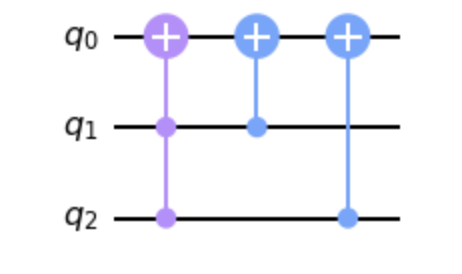
\includegraphics[scale=0.7]{reversibleOr.png}
\end{center}

\noindent This implementation was manually produced using a standard synthesis algorithm for reversible
circuits~\cite{10.1145/775832.775915}. To gain some intuition, we trace the evaluation of the circuit for input
\verb|011|. In this context, the most significant bit is at index 0. Thus the first \verb|ccx| gate negates \verb|q[0]|
since both \verb|q[1]| and \verb|q[2]| are true producing \verb|111|; the following \verb|cx| gate produces \verb|011|; finally the last \verb|cx| produces the result \verb|111|.

There is wealth of manual and algorithmic approaches for such synthesis problems each optimizing along  different dimensions~\cite{maslov:2003:rls:1087512,1201583}. Here is the circuit produced using an approach that analyzes the recursive structure of the circuit (and would generalise to computing the disjunction of more than two inputs):

\begin{center}
  \begin{minipage}[c]{0.4\linewidth}
\begin{verbatim}
reversibleOr2.qasm:

  // setup
  cx  q[1], q[0];
  x   q[1];
  ccx q[1], q[2], q[0];
  x   q[1];
  // measure
  \end{verbatim}
  \end{minipage}
  \qquad
  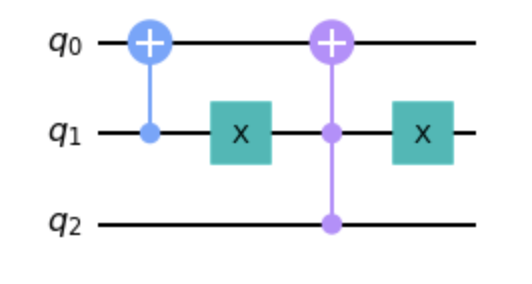
\includegraphics[scale=0.7]{reversibleOr2.png}
\end{center}

\noindent The evaluation of this circuit prints the same truth table as above confirming their equivalence. Tracing the
evaluation on the same input value \verb|011| goes through the stages \verb|111|, \verb|101|, \verb|101|, and finally \verb|111|.

The situation for Shor's algorithm is just as described above but with a more involved function of the form $f(r) = a^{r} \mod N$ for fixed $a$ and $N$. The specification of the circuit is relatively straightforward to calculate. Here it is for $a=11$ and $N=15$:
\[\begin{array}{rcll}
g(r,h) &=& \left\{ \begin{array}{ll}
                     (r,h+1) & \mbox{when~$r$~even~and~$h$~even} \\
                     (r,h-1) & \mbox{when~$r$~even~and~$h$~odd} \\
                     (r,11-h) & \mbox{when~$r$~odd~and~$4 > h \geq 0$~or~$12 > h \geq 8$} \\
                     (r,19-h) & \mbox{when~$r$~odd~and~$8 > h \geq 4$~or~$16 > h \geq 12$}
                                \end{array}\right.
\end{array}\]

\noindent However, as explained in standard accounts of the algorithm (e.g., the Qiskit implementation), producing an efficient
modular exponentiation circuit from this specification  is not straightforward and is actually the bottleneck in Shor’s algorithm. Typical
derivations of the circuit start from elementary gates, build a circuit for reversible disjunction and conjunction of
booleans, a circuit for a half-adder, a circuit for computing the carry, progressing to a circuit for modular addition,
which is used to build a circuit for modular multiplication, and then finally a circuit for modular exponentiation
taking care at each step to avoid the exponential blowup (e.g., by implementing exponentiation by squaring instead of repeated
multiplication)~\cite{shorefficient}.
